\begin{frame}
	\frametitle{Allgemeine Betrachtungen}
	\framesubtitle{Zu graphischen Bedienoberflächen}
	\begin{itemize}
		\item Interaktiv, nutzerfreundlich und komfortabel
		\item Haben sich in Software-Systemen durchgesetzt
		\item Heutige Akzeptanz und Verbreitung zeigt
		\begin{itemize}
			\item Wichtiger Bestandteil von Anwendungssystemen
			\item Interaktive SW-Systeme haben sehr hohen Stellenwert
		\end{itemize}
		\item Architekturmuster {\bf MVC}
		\begin{itemize}
			\item Grundlegende strukturelle Organisation
			\item Unabhängigkeit des funktionalen Teils von
			der Bedienschnittstelle
		\end{itemize}
	\end{itemize}
\end{frame}

\begin{frame}
	\frametitle{Das MVC Muster}
	\framesubtitle{Die Komponenten}
	\begin{center}
		Teilt eine interaktive Anwendung in 3 Komponenten auf.
	\end{center}
	\begin{itemize}
		\item {\bf Model}
		\begin{itemize}
			\item Enthält die gesamte Daten, Zustands- und Anwendungslogik
			\item Zustandsänderung über Schnittstelle
			\item Benachrichtigungen über Änderungen an Beobachter
		\end{itemize}
		\item {\bf View}
		\begin{itemize}
			\item Bildschirmrepräsentation des Anwendungsobjektes
			\item Erhält Zustand und Daten direkt vom Model
		\end{itemize}
		\item {\bf Controller}
		\begin{itemize}
			\item Nimmt Eingaben des Nutzers entgegen und verarbeitet sie
		\end{itemize}
	\end{itemize}
\end{frame}

\begin{frame}
	\frametitle{Das MVC Muster}
	\framesubtitle{Die Komponenten}
	\begin{center}
		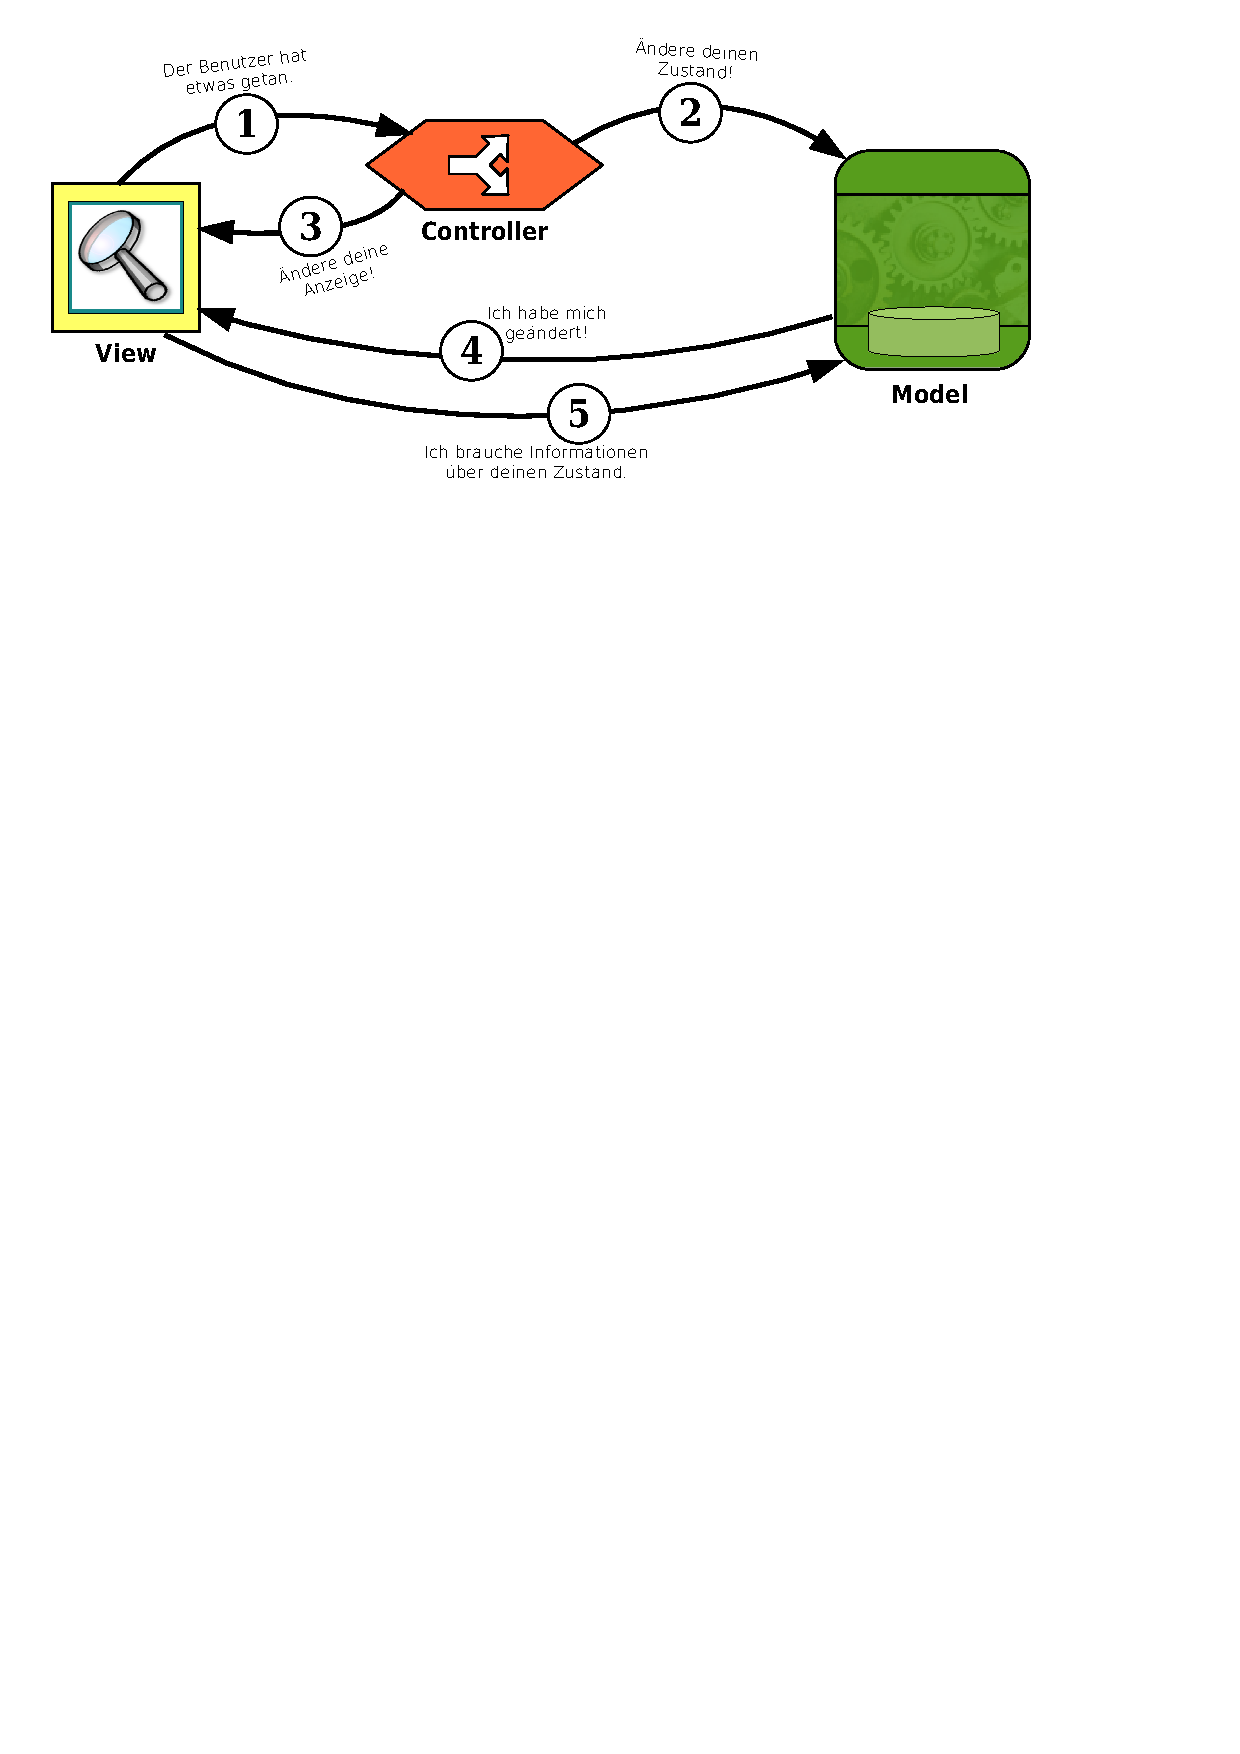
\includegraphics[trim = 0mm 207.7mm 28.6mm 0mm, clip, width=9cm]{../mvc/mvc-schema.pdf}
	\end{center}
	\begin{center}
		View- und Controller beschreiben die Bedienschnittstelle.
	\end{center}
\end{frame}

\begin{frame}
	\frametitle{MVC etwas genauer betrachtet}
	\framesubtitle{Das Observer-Muster}
	\begin{center}
		 Wichtigstes Muster für Verständnis des MVC.
	\end{center}
	\begin{itemize}
		\item {\bf Zweck}
		\begin{itemize}
			\item Definiere eine 1-zu-n-Abhängigkeit, zwischen Objekten, so dass die Änderung des
			Zustands eines Objektes dazu führt, dass alle abhängigen Objekte benachrichtigt
			und automatisch aktualisiert werden.
		\end{itemize}
	\end{itemize}
\end{frame}

\begin{frame}
	\frametitle{MVC etwas genauer betrachtet}
	\framesubtitle{Das Observer-Muster}
	\begin{center}
		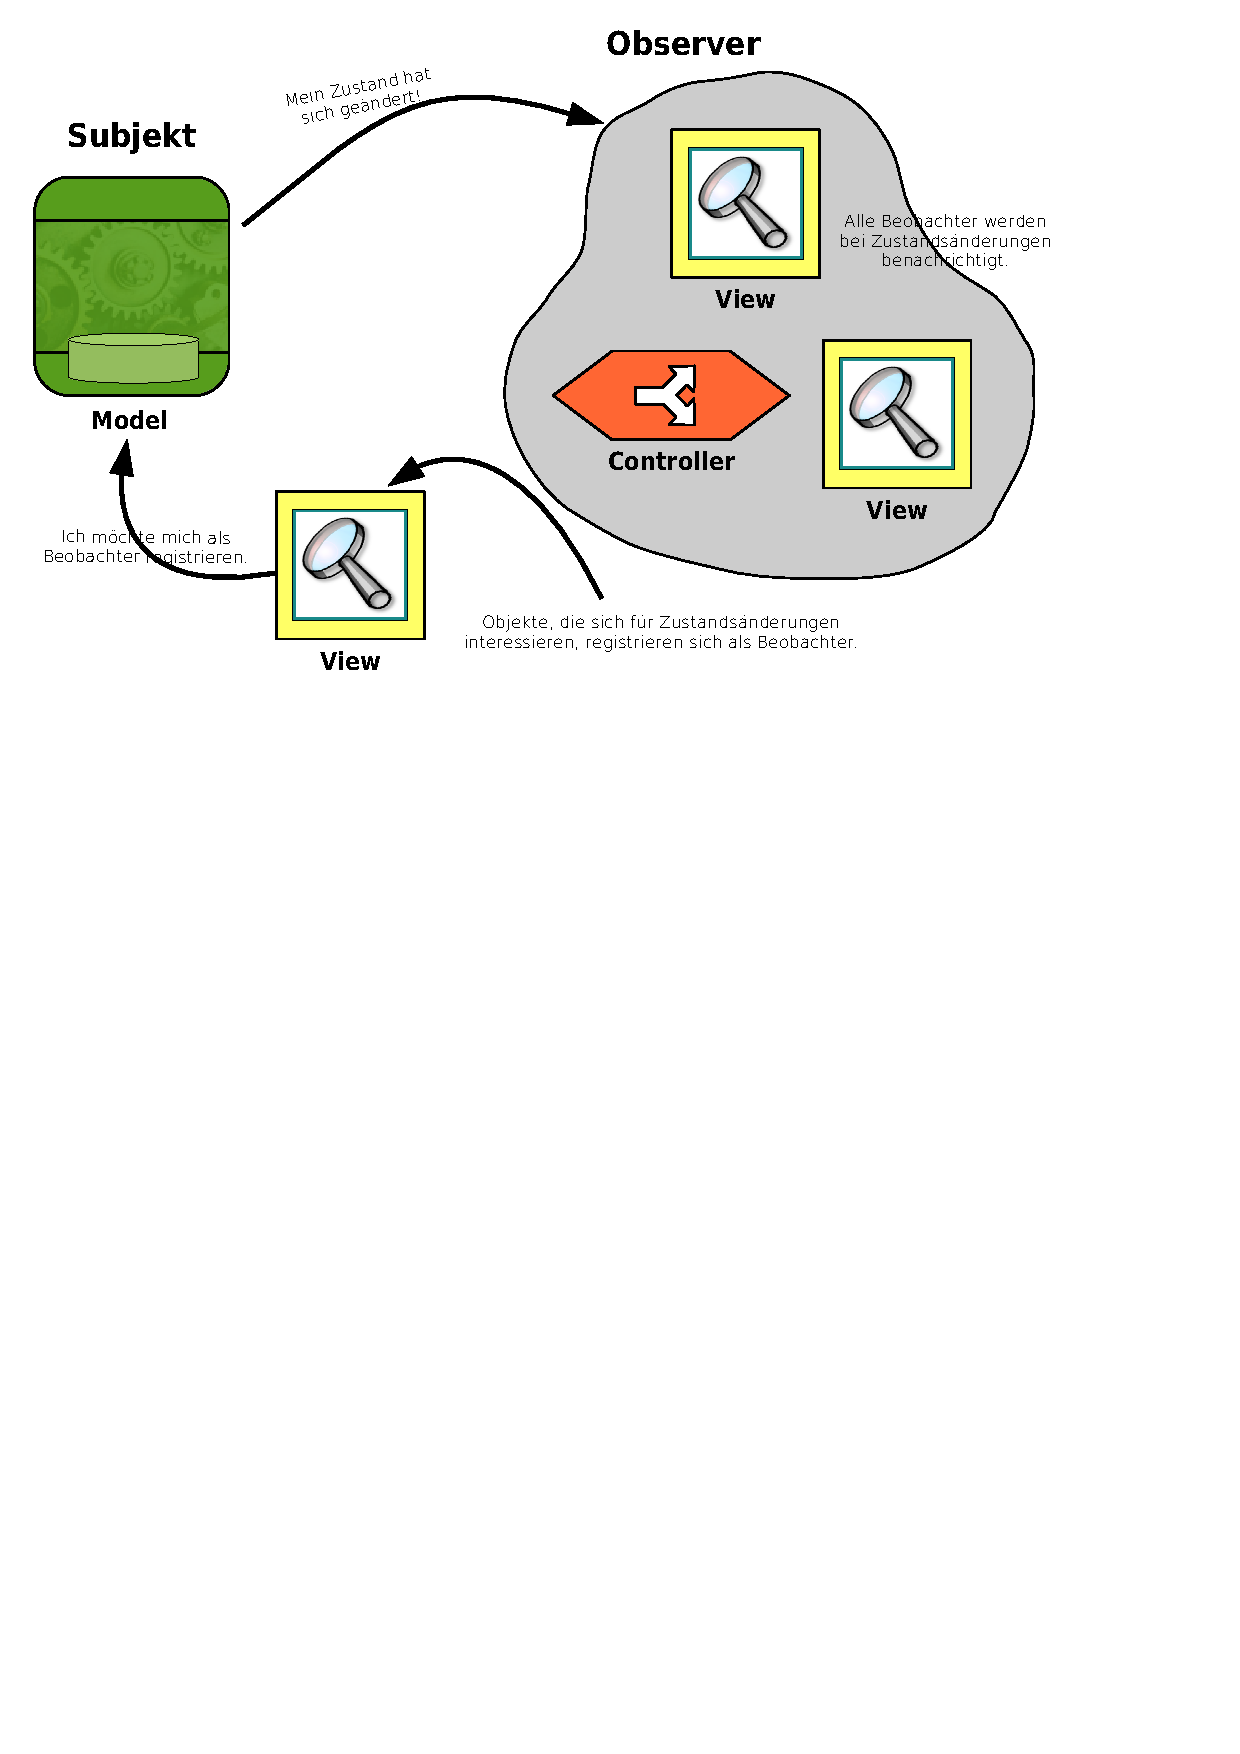
\includegraphics[trim = 0mm 176.8mm 28.6mm 0mm, clip, width=9cm]{../mvc/observer-schema.pdf}
	\end{center}
	\begin{center}
		Es macht das Model völlig unabhängig von View und Controller.
	\end{center}	
\end{frame}

\begin{frame}
	\frametitle{MVC etwas genauer betrachtet}
	\framesubtitle{Das Observer-Muster als Klassendiagramm}
	\begin{center}
		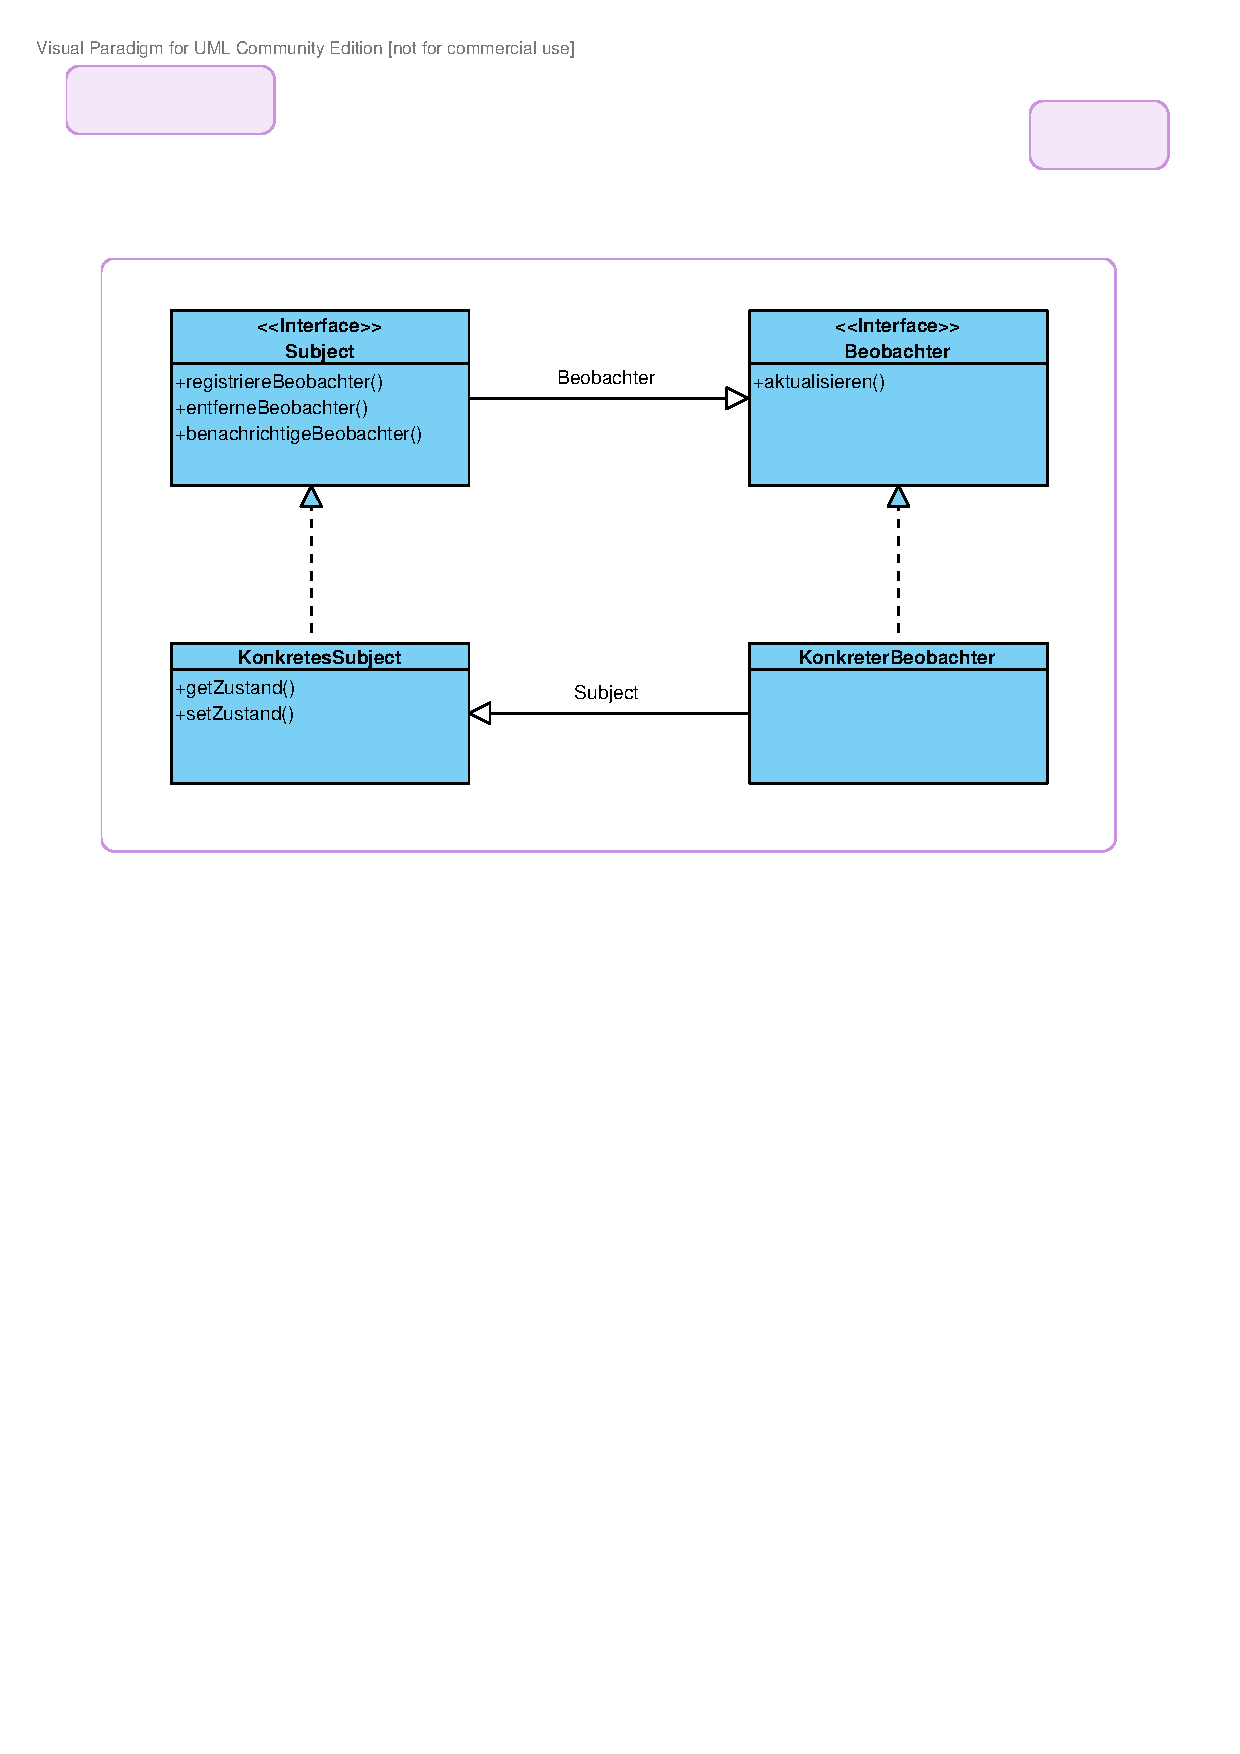
\includegraphics[trim = 18mm 155mm 22mm 45mm, clip, width=8cm]{../mvc/observer-kd.pdf}
	\end{center}	
	\begin{itemize}
		\item Beobachter registriert sich beim Subjekt
		\item Subjekt fügt es Liste seiner Beobachter hinzu
		\item Subjekt benachrichtigt alle registrierten Beobachter
		\item Subjekt bietet Zugriff über Schnittstelle an
	\end{itemize}
\end{frame}

\begin{frame}
	\frametitle{MVC etwas genauer betrachtet}
	\framesubtitle{Das Strategy-Muster}
	\begin{center}
	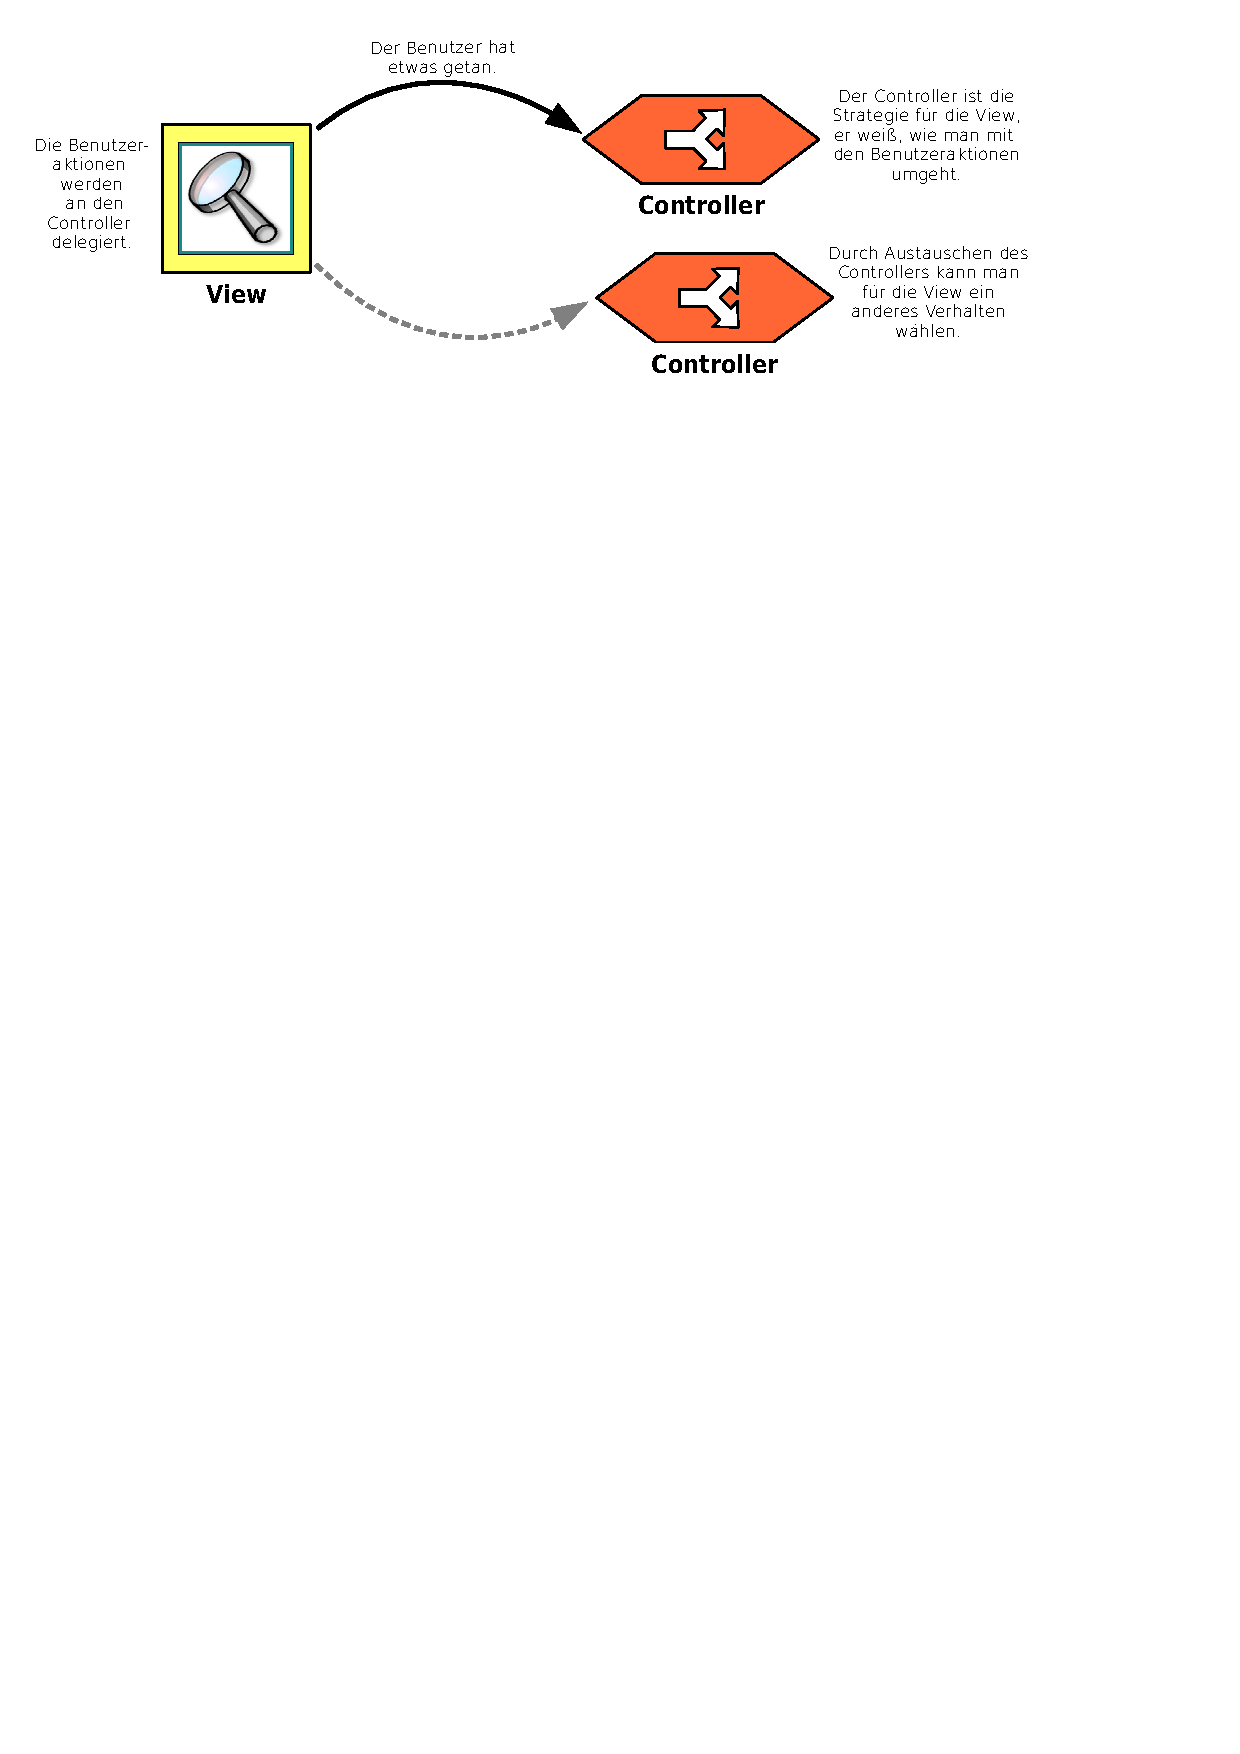
\includegraphics[trim = 0mm 227.7mm 28.6mm 0mm, clip, width=9cm]{../mvc/strategy-schema.pdf}
	\end{center}	
	\begin{itemize}
		\item View ist mit einer Strategie konfiguriert
		\item Controller ist das Verhalten der View
		\item Kann ausgetauscht werden
		\item View delegiert Benutzeraktionen an den Controller
	\end{itemize}
\end{frame}

\begin{frame}
	\frametitle{MVC etwas genauer betrachtet}
	\framesubtitle{Das Composite-Muster}
	\begin{center}
	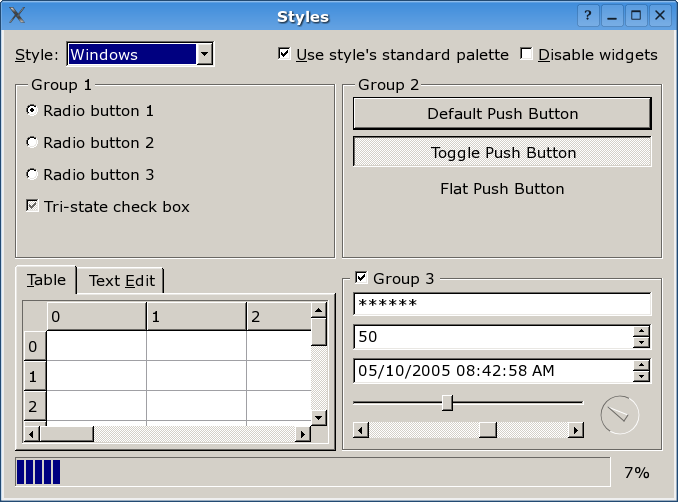
\includegraphics[width=5cm]{gui.png}
	\end{center}	
	\begin{center}
		Die GUI ist ein Kompositum.
	\end{center}
	\begin{itemize}
		\item Besteht aus Label, Buttons, Texteingabefelder, \dots
		\item Komponenten enthalten andere Komponenten
		\item Wird intern verwendet um Bestandteile der Anzeige zu verwalten
	\end{itemize}
\end{frame}


\begin{frame}
	\frametitle{Nachteile von MVC}
	\framesubtitle{In bestimmten Fällen}
	\begin{itemize}
		\item Größere Komplexität der Anwendung ohne Zugewinn an Flexibilität
		\item Potential für eine übermäßige Anzahl von Aktualisierungen
		\item Enge Verbindung zwischen View- und Controllerkomponenten
	\end{itemize}
\end{frame}

\begin{frame}
	\frametitle{Framework}
	\framesubtitle{Ein kurzer Überblick}
	\begin{itemize}
		\item Besteht aus einer Menge von zusammenarbeitenden Klassen
		\item Wiederverwendbarkeit für den Entwurf einer bestimmten Klasse
		von Software
		\item Definiert:
		\begin{itemize}
			\item Die Struktur im Großen
			\item Unterteilung in Klassen und Objekte
			\item Die jeweiligen zentralen Zuständigkeiten
			\item Zusammenarbeit und Kontrollfluß
		\end{itemize}
		\item Legt Entwursparameter im voraus fest
		\item Komponenten beinhalten Erfahrungen und sind erprobt
	\end{itemize}
\end{frame}

\begin{frame}
	\frametitle{Model/View Programmierung mit dem Qt Framework}
	\framesubtitle{Was ist Qt?}
	\begin{itemize}
		\item De facto Standard C++ Framework für die Entwicklung
		von Cross-Platform-Software
		\item Enthält Widgets mit Standard GUI-Funktionalität
		\item Open Source Edition ist Grundlage von KDE
	\end{itemize}
\end{frame}

\begin{frame}
	\frametitle{Model/View Programmierung mit Qt}
	\framesubtitle{Item Views}
	\begin{center}
		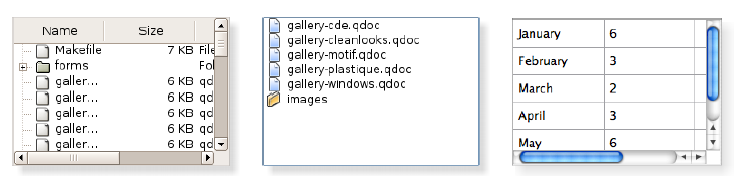
\includegraphics[width=9cm]{../mvc/qt-widgets.png}
	\end{center}
	\begin{itemize}
		\item Item-View-Widgets sind Standard GUI-Bedienungselemente
		\item List-, Tree-, Table-Views
		\item \"Aquivalente Model/View Komponenten
		\begin{itemize}
			\item {\itshape QListView}
			\item {\itshape QTableView}
			\item {\itshape QTreeView}
		\end{itemize}
	\end{itemize}
\end{frame}

\begin{frame}
	\frametitle{Model/View Programmierung mit Qt}
	\framesubtitle{Das Model/View Framework}
	\begin{itemize}
		\item Variante des MVC speziell angepaßt für Qt`s Item Views
		\item Verwendet Models um Daten anderen Komponenten zur Verfügung zu stellen
		\item Views präsentieren Daten
		\item Delegates behandeln Rendering- und Bearbeitungsprozesse
		\item Ermöglicht eine ganze Reihe Vorteile gegenüber den klassischen ItemViews
	\end{itemize}
\end{frame}

\begin{frame}
	\frametitle{Model/View Programmierung mit Qt}
	\framesubtitle{Die Model/View Architektur}
	\begin{center}
		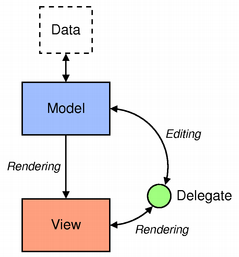
\includegraphics[width=3cm]{../mvc/modelview-overview.png}
	\end{center}
	\begin{itemize}
		\item Resultiert aus der Kombination von View und Controller in einer Komponente
		\item Dies ermöglicht einen Framework basierten Ansatz auf der Grundlage des MVC
		\item Mit Delegates kann man individuell auf Benutzereingaben reagieren
	\end{itemize}
	\begin{center}
		{\small Mit {\itshape Proxy Models} können Daten von Models transformiert werden.\\
		Dies ermöglicht Sortierung und Filterung von Daten.}
	\end{center}
\end{frame}

\begin{frame}
	\frametitle{Model/View Programmierung mit Qt}
	\framesubtitle{Die Model/View Architektur}
	\begin{itemize}
		\item {\bf Model}
		\begin{itemize}
			\item Kommuniziert mit Datenquelle
			\item Bietet Standardinterface für Zugriff der anderen Komponenten
		\end{itemize}
		\item {\bf View}
		\begin{itemize}
			\item Bekommt Model-Indizies vom Model
			\item Diese referenzieren Daten-Items
		\end{itemize}
		\item {\bf Delegate}
		\begin{itemize}
			\item Rendert die Daten-Items in View
			\item Wird Item bearbeitet werden ebenfalls Model-Indizies verwendet
		\end{itemize} 
	\end{itemize}
	\begin{center}
		Komponenten werden von abstrakten Klassen definiert, welche Standardinterfaces anbieten.
	\end{center}
\end{frame}

\begin{frame}
	\frametitle{Model/View Programmierung mit Qt}
	\framesubtitle{Die Model/View Architektur}
	\begin{center}
		{\small Kommunikation der Komponenten mittels {\itshape Signals} und 
			{\itshape Slots}\footnote{Qt-Mechanismus für die Kommunikation zwischen Objekten}.}
	\end{center}
	\begin{itemize}
		\item Signals vom Model informieren View über Datenänderungen
		\item Signals von der View bieten Informationen über Benutzeraktionen auf Daten-Items
		\item Signals vom Delegate während der Editierung verwendet, um Model und View
		über aktuellen Bearbeitungszustand zu informieren
	\end{itemize}
\end{frame}

\begin{frame}
	\frametitle{Model/View Programmierung mit Qt}
	\framesubtitle{Weitere Informationen im Internet}
	\begin{center}
		{\Large \bf http://www.qtsoftware.com}
	\end{center}
\end{frame}

